% !Mode:: "TeX:UTF-8"
%!TEX program  = xelatex

\documentclass[bwprint]{gmcmthesis}
\bibliographystyle{gmcm}
\title{全国研究生数学建模竞赛论文标题}
\baominghao{18102510035} %参赛队号
\schoolname{华东理工大学 \quad 华东师范大学}%学校名称
\membera{沈皓杰} %队员A
\memberb{李佳倩} %队员B
\memberc{张文清} %队员C
\begin{document}
 
 %生成标题
\maketitle
 
 %填写摘要
\begin{abstract}
本模板是为全国研究生数学建模竞赛编写的 \LaTeX{} 模板, 旨在让大家专注于
论文的内容写作, 而不用花费过多精力在格式的定制和调整上. 本手册是相应的参考, 其
中提供了一些环境和命令可以让模板的使用更为方便. 同时需要注意, 使用者需要有一
定的 \LaTeX{} 的使用经验, 至少要会使用 ctex 宏包的一些功能, 比如调节字距或修改字体
大小等等.


另外, 欢迎大家购买我们是视频教程,点击\href{https://item.taobao.com/item.htm?spm=a1z10.1-c.w4004-3473795048.4.ThFQCG&id=43823508044}{\fbox{这里}}。

欢迎大家到QQ群里沟通交流:91940767.

\uwave{关注我们的微信公众号}:

\centerline{\includegraphics[width=5cm]{gongzhonghao}}


\keywords{折叠桌\quad  曲线拟合\quad   非线性优化模型\quad  受力分析}
\end{abstract}

\pagestyle{plain}

%目录 不推荐加
\tableofcontents
\newpage

\section{问题重述}

\subsection{问题背景}
恐怖袭击是指极端分子或组织人为制造的、针对但不仅限于平民及民用设施的、不符合国际道义的攻击行为,它不仅具有极大的杀伤性与破坏力,能直接造成巨大的人员伤亡和财产损失,而且还给人们带来巨大的心理压力,造成社会一定程度的动荡不安,妨碍正常的工作与生活秩序,进而极大地阻碍经济的发展。

恐怖主义是人类的共同威胁,打击恐怖主义是每个国家应该承担的责任。对恐怖袭击事件相关数据的深入分析有助于加深人们对恐怖主义的认识,为反恐防恐提供有价值的信息支持。
\subsection{需要解决的问题}
现有数据如下:附件1选取了某组织搜集整理的全球恐怖主义数据库(GTD)中1998-2017年世界上发生的恐怖袭击事件的记录;附件2是有关变量的说明,节译自数据库说明文档,原文可以在http://www.start.umd.edu/gtd/中下载;附件2文档较长,附件3提供了一个内容摘要。

以此3份附件为数据基础,本文依次解决如下问题:

问题1:依据附件1以及其它有关信息,结合现代信息处理技术,借助数学建模方法建立基于数据分析的量化分级模型,将附件1给出的事件按危害程度从高到低分为一至五级,列出近二十年来危害程度最高的十大恐怖袭击事件,并给出表1中事件的分级。

% Table generated by Excel2LaTeX from sheet 'Sheet1'
\begin{table}[htbp]
	\centering
	\caption{}
	\begin{tabular}{|c|c|}
		\hline
		\multicolumn{1}{|p{6em}|}{事件编号} & \multicolumn{1}{p{2.5em}|}{危害级别} \\
		\hline
		200108110012 &  \\
		\hline
		200511180002 &  \\
		\hline
		200901170021 &  \\
		\hline
		201402110015 &  \\
		\hline
		201405010071 &  \\
		\hline
		201411070002 &  \\
		\hline
		201412160041 &  \\
		\hline
		201508010015 &  \\
		\hline
		201705080012 &  \\
		\hline
	\end{tabular}
	\label{tab:addlabel}
\end{table}%

问题2:依据事件特征发现恐怖袭击事件制造者。针对在2015、2016年度发生的、尚未有组织或个人宣称负责的恐怖袭击事件,运用数学建模方法寻找并案调查可能性,即将可能是同一个恐怖组织或个人在不同时间、不同地点多次作案的若干案件归为一类,对应的未知作案组织或个人标记不同的代号,并按该组织或个人的危害性从大到小选出其中的前5个,记为1号-5号。再对表2列出的恐袭事件,按嫌疑程度对5个嫌疑人排序,并将结果填入下表(表中样例的意思是:对事件编号为XX的事件,3号的嫌疑最大,其次是4号,最后是5号),如果认为某嫌疑人关系不大,也可以保留空格。

% Table generated by Excel2LaTeX from sheet 'Sheet1'
\begin{table}[htbp]
	\centering
	\caption{}
	\begin{tabular}{|l|l|l|l|l|l|}
		\hline
		\multicolumn{1}{|p{4em}|}{ } & \multicolumn{1}{p{2em}|}{1号嫌疑人} & \multicolumn{1}{p{2em}|}{2号嫌疑人} & \multicolumn{1}{p{2em}|}{3号嫌疑人} & \multicolumn{1}{p{2em}|}{4号嫌疑人} & \multicolumn{1}{p{2em}|}{5号嫌疑人} \\
		\hline
		\multicolumn{1}{|p{4em}|}{样例XX} & \multicolumn{1}{c|}{4} & \multicolumn{1}{c|}{3} & \multicolumn{1}{c|}{1} & \multicolumn{1}{c|}{2} & \multicolumn{1}{c|}{5} \\
		\hline
		201701090031 &       &       &       &       &  \\
		\hline
		201702210037 &       &       &       &       &  \\
		\hline
		201703120023 &       &       &       &       &  \\
		\hline
		201705050009 &       &       &       &       &  \\
		\hline
		201705050010 &       &       &       &       &  \\
		\hline
		201707010028 &       &       &       &       &  \\
		\hline
		201707020006 &       &       &       &       &  \\
		\hline
		201708110018 &       &       &       &       &  \\
		\hline
		201711010006 &       &       &       &       &  \\
		\hline
		201712010003 &       &       &       &       &  \\
		\hline
	\end{tabular}%
	\label{tab:addlabel}%
\end{table}%

问题3:依据附件1并结合因特网上的有关信息,建立适当的数学模型,研究近三年来恐怖袭击事件发生的主要原因、时空特性、蔓延特性、级别分布等规律,进而分析研判下一年全球或某些重点地区的反恐态势,用图表给出你们的研究结果,提出你们对反恐斗争的见解和建议。

问题4 给出模型和方法,通过数学建模进一步挖掘附件1数据的作用。


\subsubsection{问题的提出内容一}

围绕创意平板折叠桌的动态变化过程、设计加工参数,本文依次提出如下问题:

(1)给定长方形平板尺寸 ($120 cm \times 50 cm \times 3 cm$),每根木条宽度(2.5 cm),连接桌腿木条的钢筋的位置,折叠后桌子的高度(53 cm)。要求建立模型描述此折叠桌的动态变化过程,并在此基础上给出此折叠桌的设计加工参数和桌脚边缘线的数学描述。



(2)折叠桌的设计应做到产品稳固性好、加工方便、用材最少。对于任意给定的折叠桌高度和圆形桌面直径的设计要求,讨论长方形平板材料和折叠桌的最优设计加工参数,例如,平板尺寸、钢筋位置、开槽长度等。对于桌高70 cm,桌面直径80 cm的情形,确定最优设计加工参数。


(3)给出软件设计的数学模型,可以根据客户任意设定的折叠桌高度、桌面边缘线的形状大小和桌脚边缘线的大致形状,给出所需平板材料的形状尺寸和切实可行的最优设计加工参数,使得生产的折叠桌尽可能接近客户所期望的形状,并根据所建立的模型给出几个设计的创意平板折叠桌。要求给出相应的设计加工参数,画出至少8张动态变化过程的示意图。

\section{模型的假设}

\begin{itemize}
\item 高维数据(样本)位于一个维数比数据空间维数小得多的流形上;
\item 假设受害者的国籍对恐怖袭击事件的危害程度分级没有影响;

\end{itemize}

\section{符号说明}

\begin{tabular}{cc}
 \hline
 \makebox[0.4\textwidth][c]{符号}	&  \makebox[0.5\textwidth][c]{意义} \\ \hline
 D	    & 木条宽度(cm) \\ \hline
 L	    & 木板长度(cm)  \\ \hline
 W	    & 木板宽度(cm)  \\ \hline
 N	    & 第n根木条  \\ \hline
 T	    & 木条根数  \\ \hline
 H	    & 桌子高度(cm)  \\ \hline
 R	    & 桌子半径(cm)  \\ \hline
 R	    & 桌子直径(cm)  \\ \hline
\end{tabular}

\section{问题一}

\subsection{问题分析及模型建立}
问题一要求基于附件1给出的恐怖袭击事件记录数据,通过量化分析,将事件按危害程度从高到低分为一至五级。由于附件提供的数据维数很高,数据结构比较复杂,难以将其直观地与恐怖袭击事件的危害程度联系起来。然而对上述数据进行分析时,并非所有属性对随后进行的数据处理都是重要的。高维数据中的信息往往包含在一个或几个低维结构中,可以用少量的简单变量来支配。


\subsection{问题求解}
题目要求从折叠桌的稳固性好、加工方便、用材最少三个角度,确定设计加工参数。我们可以从应力、支撑面积考虑稳固性,从开槽长度考虑加工方便,从木板长度考虑用材最少。而它们之间又是相互制约,我们需要确定最优设计加工参数,可以建立非线性规划模型,用lingo软件来求解最优设计加工参数(平板尺寸、钢筋位置、开槽长度等),这里以合力的方向(斜向上)与最长木条(桌腿)的夹角方向最小为目标函数,以木条所承受应力小于木条的许用应力、支撑面积大于桌面面积、木条的开槽长度小于木条本身长为约束条件。
\begin{figure}[!h]
\centering
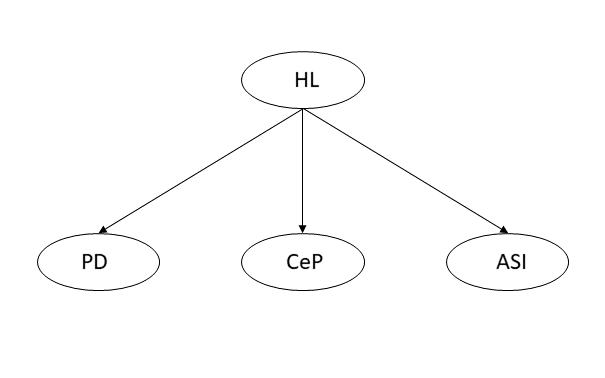
\includegraphics[width=.7\textwidth]{1.png}
\caption{问题三流程图}
\end{figure}
\section{问题二}
题目要求制作软件的意思就是客户给定折叠桌高度、桌面边缘线的形状大小和桌脚边缘线的大致形状,将这些信息输入程序就得到客户想要的桌子。我们在求解最优设计加工参数时,自行给定桌面边缘线形状(椭圆、相交圆等),桌脚边缘线形状,折叠桌高度,应用第二问的非线性规划模型,用MATLAB软件绘制折叠桌截面图,得到自己设计的创意平板折叠桌。

\section{问题三}
\section{问题四}



%参考文献   手工录入
%\begin{thebibliography}{9}%宽度9
% \bibitem{bib:one} ....
% \bibitem{bib:two} ....
%\end{thebibliography}

%采用bibtex方案

%\cite{mittelbach_latex_2004,wright_latex3_2009,beeton_unicode_2008,vieth_experiences_2009}
\bibliography{example}

\newpage
%附录
\appendix
%\setcounter{page}{1} %如果需要可以自行重置页码。
\section{我的 MATLAB 源程序}
\begin{lstlisting}[language=Matlab]%设置不同语言即可。
kk=2;[mdd,ndd]=size(dd);
while ~isempty(V)
[tmpd,j]=min(W(i,V));tmpj=V(j);
for k=2:ndd
[tmp1,jj]=min(dd(1,k)+W(dd(2,k),V));
tmp2=V(jj);tt(k-1,:)=[tmp1,tmp2,jj];
end
tmp=[tmpd,tmpj,j;tt];[tmp3,tmp4]=min(tmp(:,1));
if tmp3==tmpd, ss(1:2,kk)=[i;tmp(tmp4,2)];
else,tmp5=find(ss(:,tmp4)~=0);tmp6=length(tmp5);
if dd(2,tmp4)==ss(tmp6,tmp4)
ss(1:tmp6+1,kk)=[ss(tmp5,tmp4);tmp(tmp4,2)];
else, ss(1:3,kk)=[i;dd(2,tmp4);tmp(tmp4,2)];
end;end
dd=[dd,[tmp3;tmp(tmp4,2)]];V(tmp(tmp4,3))=[];
[mdd,ndd]=size(dd);kk=kk+1;
end; S=ss; D=dd(1,:);


 \end{lstlisting}


\end{document} 